\documentclass[a4paper, 12pt]{article}
\usepackage[latin1]{inputenc}
\usepackage[english]{babel}
\usepackage[T1]{fontenc}
\setcounter{section}{0}
\setcounter{figure}{0}
\usepackage{graphicx}
\usepackage{float}
\usepackage[centertags]{amsmath}
\usepackage{amsfonts}
\usepackage{amsthm}
\usepackage{newlfont}

\usepackage{footnote}

\usepackage{fancyhdr}
\usepackage{tesisty}
\usepackage{enumitem}
\setlist[itemize]{noitemsep, leftmargin=10pt}
\usepackage{amssymb}
\usepackage{listings}
\usepackage{hyperref} 
\usepackage{lipsum}
\usepackage[framed,numbered,autolinebreaks,useliterate]{mcode}
\lstset{language=Matlab, basicstyle=\scriptsize\ttfamily, frame=single}
%\lstloadlanguages{Matlab}
%\usepackage{rotating}

%-------------------------------
% DEFINIZIONE DEGLI ENVIRONMENT
%-------------------------------

\newtheorem{obs}{Osservazione}[section]
\newenvironment{oss}
    {\begin{obs}\begin{normalfont}}
    {\hfill $\square \!\!\!\!\checkmark$ \end{normalfont}\end{obs}}

\newtheorem{pro}{Problema}[section]
\newenvironment{prob}
    {\begin{pro}\begin{normalfont}}
    {\hfill $\spadesuit$ \end{normalfont}\end{pro}}

\newtheorem{teor}{Teorema}[section]
\newenvironment{teorema}
    {\begin{teor}\textit }
    {\hfill  \end{teor}}

\newtheorem{defn}{Definizione}[section]
\newenvironment{de}
    {\begin{defn}\begin{normalfont}}
    {\hfill $\clubsuit$ \end{normalfont}\end{defn}}

%-----------------------------
% CONFIGURAZIONE DELLA PAGINA
%-----------------------------

\hfuzz2pt % Don't bother to report over-full boxes if over-edge is < 2pt

\fancypagestyle{plain}{
\fancyhead{}\renewcommand{\headrulewidth}{0pt} } \pagestyle{fancy}
%\renewcommand{\chaptermark}[1]{\markboth{\small CAP. \thechapter \textit{ #1}} {} }
\renewcommand{\sectionmark}[1]{\markright{\small  \thesection \textit{ #1}} {} }
\voffset=-20pt    % distanza tra il limite superiore del foglio e l'intestazione
\headsep=40pt     % distanza  l'intestazione ed il testo del corpo
\hoffset=0 pt     % misura equivalente al margine sinistro
\textheight=620pt % altezza del corpo del testo
\textwidth=435pt  % larghezza del corpo del testo
\footskip=40pt    % distanza tra il testo del corpo ed il pie' di pagina
\fancyhead{}      % cancella qualsiasi impostazione per l'intestazione
\fancyfoot{}      % cancella qualsiasi impostazione per il pie' di pagina
\headwidth=435pt  % larghezza del'intestazione e del pie' di pagina
\fancyhead[R]{}%{\rightmark} \fancyfoot[L]{\leftmark}
\fancyfoot[R]{}%{\thepage}
\renewcommand{\headrulewidth}{0.3pt}   % spessore della linea dell'intestazione
\renewcommand{\footrulewidth}{0.3pt}   % spessore della linea del pi�di pagina

\numberwithin{equation}{section}
\renewcommand{\theequation}{\thesection.\arabic{equation}}
%--------------------------
% MODIFICARE DA QUI IN POI
%--------------------------

\begin{document}
\corso{Artificial Intelligence} \titoloTesi{} \anno{2015/2016}

\baselineskip=25pt

\intestazione

%------------------------------------------------
% INTRODUZIONE E RINGRAZIAMENTI (NON MODIFICARE)
%------------------------------------------------

\fancypagestyle{plain}{
\fancyhead\renewcommand{\headrulewidth}{0pt} } \pagestyle{fancy}
%\renewcommand{\chaptermark}[1]{\markboth{\small Cap. \thechapter \textit{ #1}} {} }
\renewcommand{\sectionmark}[1]{\markright{\small  \S \thesection \textit{ #1}} {} }
\voffset=-20pt                         % distanza tra il limite superiore del foglio e l'intestazione
\headsep=40pt                          % distanza  l'intestazione ed il testo del corpo
\hoffset=0pt                           % misura equivalente al margine sinistro
\textheight=620pt                      % altezza del corpo del testo
\textwidth=435pt                       % larghezza del corpo del testo
\footskip=40pt                         % distanza tra il testo del corpo ed il pie' di pagina
\fancyhead{}                           % cancella qualsiasi impostazione per l'intestazione
\fancyfoot{}                           % cancella qualsiasi impostazione per il pie' di pagina
\headwidth=435pt                       % larghezza del'intestazione e del pie' di pagina
\fancyhead[R]{\rightmark} \fancyfoot[L]{\leftmark}
\fancyfoot[R]{\thepage}
\renewcommand{\headrulewidth}{0.3pt}   % spessore della linea dell'intestazione
\renewcommand{\footrulewidth}{0.3pt}   % spessore della linea del pié di pagina

\pagenumbering{Roman} \tableofcontents
\newpage

\pagenumbering{arabic}

\fancyhead[R]{Introduzione} \fancyfoot[L]{Introduzione}
\fancyfoot[R]{\thepage}


\fancyhf{} %elimina header/footer vecchi


\fancyhead[R]{\rightmark} \fancyhead[L]{\leftmark}
\fancyfoot[R]{\thepage}


%-----------------------
% DEFINIZIONE VARIABILI
%-----------------------

\newcommand{\figura}{figura}

%---------------------
% INCLUSIONE CAPITOLI
%---------------------

\begin{abstract}
This paper is an academic final report for the Artificial Intelligence course. The goal of the project is to implement a Ros module for building high-level representations of the environment that embody both metric and symbolic knowledge about it. A key issue in the interaction with robots is to establish a proper relationship between the symbols used in the representation and the corresponding elements of the operational environment.
\end{abstract}	

\section{Introduction}

Robotics is in an exciting stage and human machine interaction is being intensively studied.
Robots are expected to get closely involved into human life as they are being marketed for commercial applications such as telepresence, service or entertainment. However, although they are expected to become consumer products, there is still a gap in terms of user expectations and robot functionalities. A key limiting factor is the lack of awareness of the robot on the operational environment.
This project investigates several strategies to integrate a knowledge base in the ROS framework. The implemented system provides knowledge processing capabilities that combine knowledge representation and reasoning methods to manipulate and interact with physical objects of the operational milieu through an \textit{API system} and a graphical interface.\\

\subsection{Objectives}
\label{sec:objectives}

\begin{enumerate}
\item Integrate a knowledge base in ROS,
\item Create a node to Parse owl files in ROS environment,
\item Consistency check of ontology,
\item Reasoner invocation,
\item Make the ROS environment aware of object's instances,
\item Graphical representation of the objects in the scene,
\item Insert new instance of object in the scene and check for consistency,
\item Delete instance and check for consistency,
\item List instances,
\item Graphical Scene configuration from Gazebo and automatic Abox update
\item Export current Abox in owl or different formats.
\end{enumerate}

\subsection{Project Schedule}
A public git repository is available at the following \href{https://github.com/GiovanniBalestrieri/JinchiMiru}{Github page}\footnote{https://github.com/GiovanniBalestrieri/JinchiMiru} and a step by step guide has been published at www.userk.co.uk\footnote{More further information visit http://userk.co.uk/handling-ontologies-with-ros/}.
\small
\noindent 
\begin{center}
\makesavenoteenv{tabular}
    \begin{tabular}{ | l | p{4cm} | p{4cm} | p{5cm} |}
    \hline
    Week & General Task & Documentation & Implementation \\ \hline
    1 &  \begin{itemize} 
    \item Perform a literature review on the previous HuRIC
     publications
     \end{itemize} & 
	\begin{itemize}
     \item  Knowledge representation and Reasoning \cite{bib11}
     \item  Huric papers
      \cite{bib1},\cite{bib2},\cite{bib3},\cite{bib4}, \cite{bib5}
	\end{itemize} & \\ \hline
    2 & \begin{itemize}
     \item Literature review of ROS compatible triple store
     \item ROS compatible simulation environments
	\end{itemize}     
     & \begin{itemize}
     \item ROS Documentation \cite{bib6}, \cite{bib7}
     \item ROS compatible simulation environments \cite{bib8}, \cite{bib9}
	\end{itemize}   & 
	\begin{itemize} 
	\item Set up ROS environment.
	\item Brainstorm Software Architecture
	\end{itemize}\\ \hline
    3 & \begin{itemize}
     \item Literature review of RDFlib based papers
     \item Test of Gazebo Simulator
     \end{itemize}  & 
     \begin{itemize}
     \item Full Training session on Gazebo Simulator \cite{bib10} 
     \item Python library RDFLib test 
     \end{itemize} & 
     \begin{itemize}
     \item Test Json Parser node
     \item Populate a scene from json files. 
     \end{itemize} \\ \hline
    4 & \begin{itemize}
     \item Kinect pointcloud literature review
     \item Object recognition papers review
     \end{itemize}  & 
     \begin{itemize}
     \item PointCloudLibrary documentation \cite{bib16}
     \item Python SciPy library classifier documentation
     \end{itemize}
      & \begin{itemize}
     \item Parse test KnowledgeBase owl file with RDFLib
     \item Clear scene script in Gazebo.
     \end{itemize}  \\
    \hline
    5 & \begin{itemize}
     \item Integrate classification algorithms
     \item Optimize python code and ROS environment.
     \end{itemize} 
     & \begin{itemize}
     \item ROS + PCL integration
     \item RDF library deep inspection
     \end{itemize} 
      & \begin{itemize}
     \item Analyze pointcloud from kinect
     \item Scene analysis, plane segmentation
     \item Object recognition, vote classifier
     \end{itemize}  \\
    \hline
    6 & \begin{itemize}
     \item Owl Reasoner integration
     \item Test RDFlib and Apache Jena
     \end{itemize} 
     & \begin{itemize}
     \item RDF lib documentation
     \item Apache Jena Fuseki Documentation \cite{bib15}
     \end{itemize} 
      & \begin{itemize}
     \item Create init node
     \item Spawn models script
     \item Remove models script
     \item Apache Jena basic setup
    \end{itemize}  \\
    \hline
    \end{tabular}
\end{center}


\begin{center}
\makesavenoteenv{tabular}
    \begin{tabular}{ | l | p{4cm} | p{4cm} | p{5cm} |}
    \hline
    Week & General Task & Documentation & Implementation \\ \hline
    7 & \begin{itemize}
     \item Consistency check
     \item RosJava integration
     \item Jena Ontology Api
     \end{itemize} 
     & \begin{itemize}
     \item RosJava guidelines \cite{bib12}
     \item Apache Jena Ontology Api \cite{bib13}
     \end{itemize} 
      & \begin{itemize}
     \item Integrate RosJava in Ros.
     \item Follow Jena Ontology Api tutorial. Basic rdf manipulation
    \end{itemize}  \\
    \hline
    8 & \begin{itemize}
     \item Consistency check
     \end{itemize} 
     & \begin{itemize}
     \item RosJava guidelines \cite{bib12}
     \item Jena Reasoner Documentation \cite{bib14}
     \end{itemize} 
      & \begin{itemize}
     \item Implement consistency check with Jena.
     \item Integrate Jena libraries in ROS
     \item Reasoner invocation in ROS.
    \end{itemize}  \\
    \hline
    9 & \begin{itemize}
     \item Owl A-box extraction
     \item Specialize Reasoner on Tbox
     \end{itemize} 
     & \begin{itemize}
     \item RDFlib export documentation     
     \item Jena Reasoner documentation     
     \end{itemize}
      & \begin{itemize}
     \item Implement A-box generator Jena
     \item Retrieve information about instances     
    \end{itemize}  \\
    \hline
    10 & \begin{itemize}
     \item Get info about model in Gazebo 
     \item Specialize Reasoner on Tbox
     \end{itemize} 
     & \begin{itemize}
     \item Programming Robots with Ros \cite{bib9}      
     \item Gazebo Documentation \cite{bib10}    
     \end{itemize}
      & \begin{itemize}
     \item Subscribe to gazebo modelStates in ROSJava
     \item Call spawn model service from ROSJava
    \end{itemize}  \\
    \hline
    11 & \begin{itemize}
     \item SPARQL queries Add, Delete, Update, GET Instance
     \item Coordinator Node Definition
     \item Interface between Semantic Map and Gazebo Node
     \end{itemize} 
     & \begin{itemize}
     \item Jena Ontology Api Documentation \cite{bib13}      
     \item Gazebo Documentation \cite{bib10}    
     \end{itemize}
      & \begin{itemize}
     \item Jena RDF graph manipulation 
     \item Jena SPARQL Delete and Add queries 
     \item Jena SPARQL GetInstance queries 
    \end{itemize}  \\
    \hline
    
    \end{tabular}
\end{center}

\begin{center}
\makesavenoteenv{tabular}
    \begin{tabular}{ | l | p{4cm} | p{4cm} | p{5cm} |}
    \hline
    Week & General Task & Documentation & Implementation \\ \hline
    12 & \begin{itemize}
     \item Test Case validation
     \item Use Case validation
     \item Application Demo
     \end{itemize} &
      & \begin{itemize}
     \item Testing of real world scenario
     \item Bug fixing 
     \item Extern Node definition
    \end{itemize}  \\
    \hline
    \end{tabular}
\end{center}
 



\section{The Ontology}
It is expected that mobile robots undertake various tasks not only in the industrial fields such as manufacturing plants and construction sites, but also in the environment we live in.

\subsection{Tbox}
In this project a generic home domain model has been taken into account. 

\begin{figure}[H]
\centering
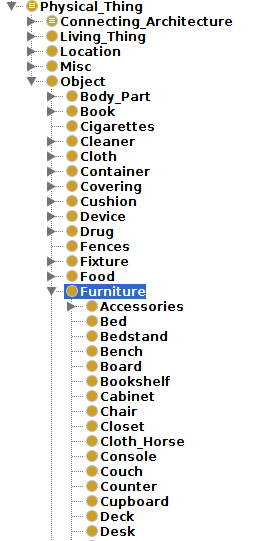
\includegraphics[width=0.3\textwidth]{imgs/ontology.png}
\label{fig:ontologyThings}
\caption{Physical Things}
\end{figure}

The furniture class describes several objects of a generic home environment a robot can interact with.

\begin{figure}[H]
\centering
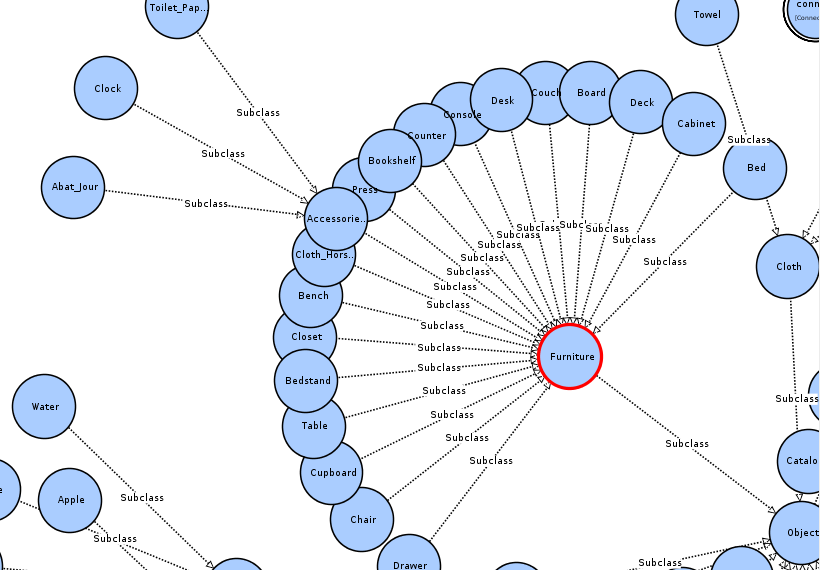
\includegraphics[width=0.8\textwidth]{imgs/ontology1.png}
\label{fig:furniture}
\caption{furniture subclasses}
\end{figure}

\subsection*{Properties}
OWL distinguishes between two main categories of properties that an ontology builder may want to define:

\begin{itemize}
	\item Object properties link individuals to individuals.
	\item Datatype properties link individuals to data values.
\end{itemize}

An object property is defined as an instance of the built-in OWL class owl:ObjectProperty. A datatype property is defined as an instance of the built-in OWL class owl:DatatypeProperty. Both owl:ObjectProperty and owl:DatatypeProperty are subclasses of the RDF class rdf:Property.\\

\subsubsection*{Properties}
The datatypes involved are shown in the Figure ~\ref{fig:datatypes} and ~\ref{fig:datatypesProtege}

\begin{figure}[H]
\centering
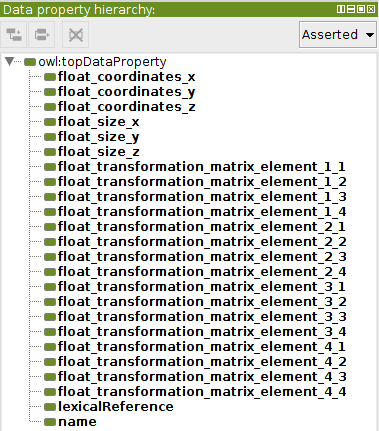
\includegraphics[width=0.6\textwidth]{imgs/datatypeProtege.png}
\label{fig:datatypesProtege}
\caption{Datatypes Visual Prot\'eg\'e}
\end{figure}

\begin{figure}[H]
\centering
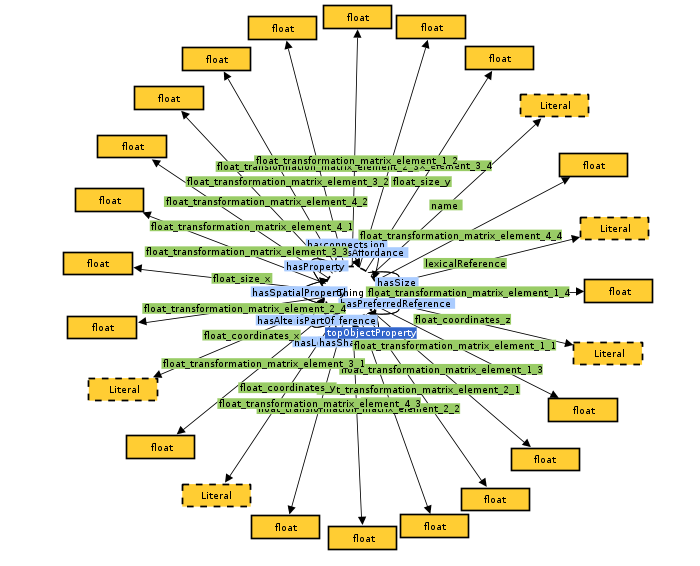
\includegraphics[width=0.6\textwidth]{imgs/Datatype.png}
\label{fig:datatypes}
\caption{Datatypes}
\end{figure}

\textit{Object Properties}

The following Figure \ref{fig:propClassTree} shows the class tree diagram of the ObjectProperties involved in the project.
\begin{figure}[H]
\centering
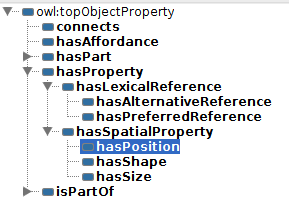
\includegraphics[width=0.6\textwidth]{imgs/propClassTree.png}
\label{fig:propClassTree}
\caption{Object Properties Class Tree}
\end{figure}

As an example, consider the following set of owl statements about the ObjectProperty hasPosition. This property is of the type IrreflexivePropery and is a subProperty of SpacialProperty.


\begin{lstlisting}
<owl:ObjectProperty rdf:about="sm#hasPosition">
    <rdfs:subPropertyOf rdf:resource="sm#hasSpatialProperty"/>
    <rdf:type rdf:resource="http://www.w3.org/2002/07/owl#IrreflexiveProperty"/>
</owl:ObjectProperty>
\end{lstlisting}    

Let us consider another Property involved in this project.

\begin{lstlisting}
<owl:Class rdf:about="sm#Coordinates">
    <rdfs:subClassOf rdf:resource="sm#Position"/>
    <rdfs:subClassOf>
       <owl:Restriction>
           <owl:onProperty rdf:resource="sm#float_coordinates_z"/>
           <owl:someValuesFrom rdf:resource="http://www.w3.org/2001/XMLSchema#float"/>
           </owl:Restriction>
     </rdfs:subClassOf>
     <rdfs:subClassOf>
        <owl:Restriction>
           <owl:onProperty rdf:resource="sm#float_coordinates_x"/>
           <owl:qualifiedCardinality rdf:datatype="http://www.w3.org/2001/XMLSchema#nonNegativeInteger">1
           </owl:qualifiedCardinality>
           <owl:onDataRange rdf:resource="http://www.w3.org/2001/XMLSchema#float"/>
           </owl:Restriction>
     </rdfs:subClassOf>
     <rdfs:subClassOf>
        <owl:Restriction>
           <owl:onProperty rdf:resource="sm#float_coordinates_y"/>
           <owl:qualifiedCardinality rdf:datatype="http://www.w3.org/2001/XMLSchema#nonNegativeInteger">1
			</owl:qualifiedCardinality>
           <owl:onDataRange rdf:resource="http://www.w3.org/2001/XMLSchema#float"/>
       </owl:Restriction>
   </rdfs:subClassOf>
</owl:Class>   
\end{lstlisting}

The class Coordinates is a subclass of the class Position and of three anonymous classes. A property restriction describes an anonymous class, namely a class of all individuals that satisfy the restriction. \\\
The first restriction is a Value contraint linked (using owl:onProperty) the Property float\_coordinates\_z  to a class of all individuals for which at least one value of the property concerned is an instance of a data value in the data range.\\
The second and third restrictions are Cardinality contraints linked to the Property float\_coordinates\_x and float\_coordinates\_y.


\subsection{Abox}
The collection of individual are stored in a separate file called semantic\_mapping, the Abox. The demo supports operations on four classes of instances since the 3D environment requires tridimentional models of the object to be represented. This constrain could be relaxed by adding an exhaustive collection of 3D models and by associating them to the corresponding classes.\\

\subsubsection*{An instance of the class Chair}
Individuals are defined with individual axioms called ``facts''. These facts are statements indicating class membership of individuals and property values of individuals. As an example, consider the following set of statements about an instance of the class Chair:

\begin{lstlisting}    
<NamedIndividual rdf:about="sm#chair1">
        <rdf:type rdf:resource="&semantic_mapping_domain_model;Chair"/>
        <semantic_mapping_domain_model:hasPosition rdf:resource="sm#chair1_coordinates"/>
        <semantic_mapping_domain_model:hasSize rdf:resource="sm#chair1_size"/>
        <semantic_mapping_domain_model:hasAlternativeReference rdf:resource="sm#chair_alternative_reference_1"/>
        <semantic_mapping_domain_model:hasAlternativeReference   rdf:resource="sm#chair_alternative_reference_2"/>
        <semantic_mapping_domain_model:hasAlternativeReference  rdf:resource="sm#chair_alternative_reference_3"/>
        <semantic_mapping_domain_model:hasPreferredReference rdf:resource="sm#chair_preferred_reference"/>
    </NamedIndividual>
\end{lstlisting}

This example includes a number of facts about the individual chair1, an instance of the class Chair. The chair has three alternative references and one preferred lexical reference. These properties link a chair to a typed literal with the XML Schema datatype date. The XML schema document on datatypes contains the relevant information about syntax and semantics of this datatype. The property hasPosition and hasSize link the chair to instances of the type Coordinates and Dimensions.

The following figure shows the same information on Prot\'eg\'e:

\begin{figure}[H]
\centering
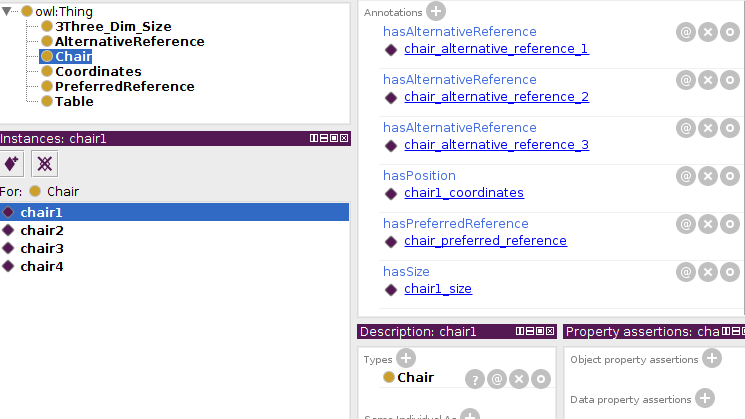
\includegraphics[width=0.6\textwidth]{imgs/chair1.png}
\label{fig:datatypes}
\caption{Chair1}
\end{figure}

\textbf{Properties}

The following example shows AlternativeReference instance property.
\begin{lstlisting}    
<NamedIndividual rdf:about="sm#chair_alternative_reference_1">
        <rdf:type rdf:resource="&semantic_mapping_domain_model;AlternativeReference"/>
        <semantic_mapping_domain_model:lexicalReference rdf:datatype="&xsd;string">chair
        </semantic_mapping_domain_model:lexicalReference>
    </NamedIndividual>
\end{lstlisting}


\begin{figure}[H]
\centering
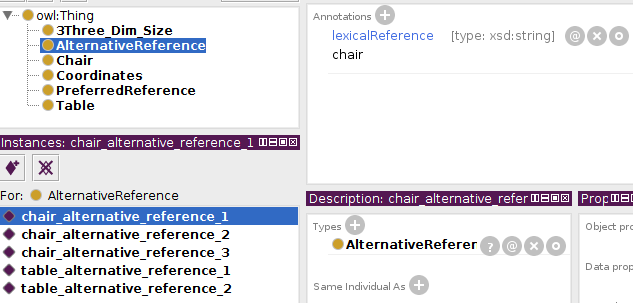
\includegraphics[width=0.6\textwidth]{imgs/refChair1.png}
\label{fig:datatypes}
\caption{Alternative Reference 1}
\end{figure}

The following example shows the instance of the 3Three\_Dim\_Size property associated to the individual chair1
\begin{lstlisting}    
<NamedIndividual rdf:about="sm#chair1_coordinates">
        <rdf:type rdf:resource="&semantic_mapping_domain_model;Coordinates"/>
        <semantic_mapping_domain_model:float_coordinates_z rdf:datatype="&xsd;float">0.0
        </semantic_mapping_domain_model:float_coordinates_z>
        <semantic_mapping_domain_model:float_coordinates_y rdf:datatype="&xsd;float">0.0
        </semantic_mapping_domain_model:float_coordinates_y>
        <semantic_mapping_domain_model:float_coordinates_x rdf:datatype="&xsd;float">1.0
        </semantic_mapping_domain_model:float_coordinates_x>
    </NamedIndividual>
\end{lstlisting}



\begin{figure}[H]
\centering
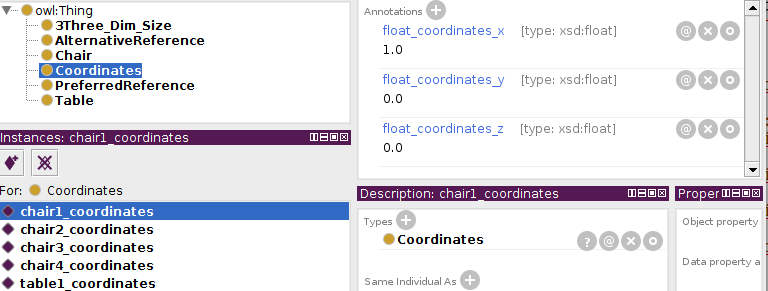
\includegraphics[width=0.6\textwidth]{imgs/coordchair1.png}
\label{fig:datatypes}
\caption{Coordinates chair 1}
\end{figure}


\section{Involved Technologies}

\subsection{JENA Ontology API}
There are several languages available for representing ontology information on the semantic web. They range from the most expressive, OWL Full, through to the weakest, RDFS. With RDFS it is possible to build a simple hierarchy of concepts, and a hierarchy of properties. The ontology language used in this project is the OWL FULL. OWL language allows properties to be denoted as transitive, symmetric or functional, and allows one property to be declared as the inverse of another.\\
\\
The Jena ontology API is a Java programming toolkit. Jena's support is limited to ontology formalisms built on top of RDF. One of the key benefits of building an ontology-based application is using a reasoner to derive additional truths about the concepts you are modelling. Jena includes support for a variety of reasoners through the inference API.
\\
A common feature of Jena reasoners is that they create a new RDF model which appears to contain the triples that are derived from reasoning as well as the triples that were asserted in the base model. The ontology API can query an extended inference model and extract information not explicitly given.

\subsection{ROS Framework}
The Robot Operating System (ROS) is a framework  for writing robot software. It is a collection of tools, libraries and conventions that aims to simplify the task of creating complex and robust robot behavior across a wide variety of robotics platforms. 
ROS was built from the ground up to encourage collaborative robotics software development. A ROS system consists of a large number of modules that pass data to one another using a inter-process communication. Each node sends and receives information to and from other nodes of the system using \textit{Topics}.
\\
\begin{figure}[H]
\centering
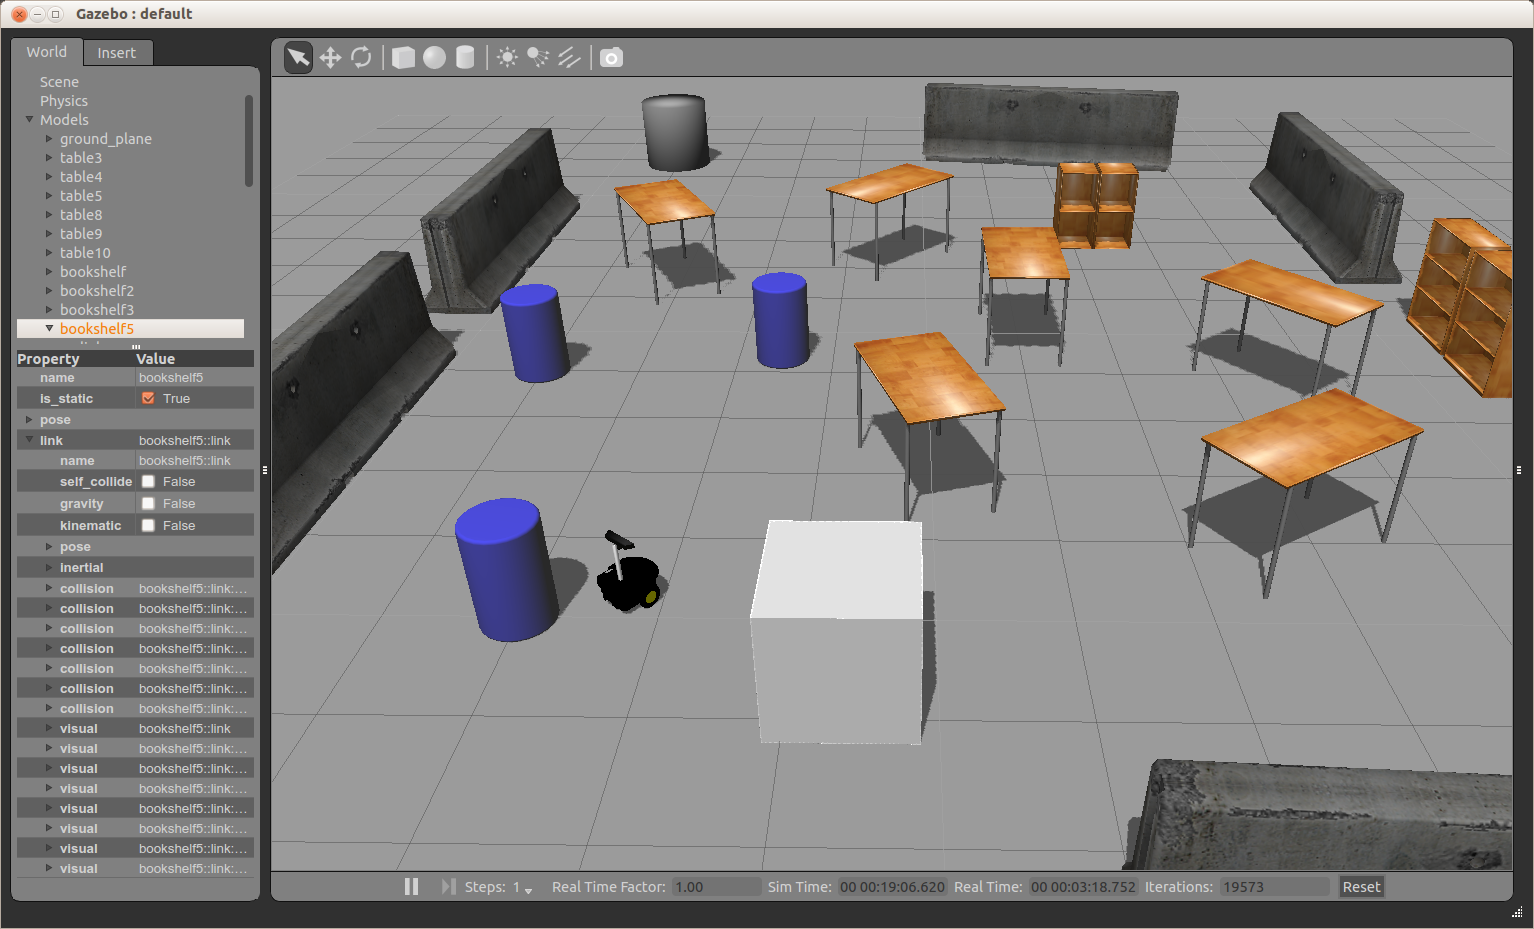
\includegraphics[width=0.8\textwidth]{imgs/gazebo1.png}
\label{fig:gazebo1}
\caption{ROS simulation}
\end{figure}

It is a tools-based program. Tasks such as visualizing the system interconnections generating documentation, logging data, filtering sensor's data, etc. are all performed by separate programs. The individual tools themselves are relatively small and generic. There is no central routing service.
\\
ROS chose a multilingual approach that allows programmers to accomplish tasks using scripting languages such as Python and MATLAB or using faster ones like C++. Client libraries exist for LISP, Java, JavaScript, Ruby,R and others. ROS libraries communicate with one another by following a convention that describes how messages are serialized before being transmitted over the network. The ROS conventions encourages contributors to create standalone libraries in order to allow the reuse of software and speed up development.\\
\\
The core of ROS is released under the BSD license which allows commercial and noncommercial use.

\subsection{Gazebo Simulation Environment}

Robotics implies robots. Most part of these platforms are used for research purposes and are custom built to investigate a particular aspect of interest. However, there are a growing number of standard products that can be purchased and used out of the box for development and operations in many domains of robotics.\\
Although several robotics platforms are considered to be low cost they are still significant investments. Even the best robots can break periodically due to various combinations of operator error, environmental conditions, manufacturing and design defects. All of these drawbacks can be avoided, or at least minimized, by using simulated robotic structures and a simulation environment. Gazebo is a $3D$ dynamic simulator with the ability to accurately and efficiently simulate populations of robots in complex indoor and outdoor environments. It offers physics engine with high degree of fidelity and a variety of sensors.

Many robots are provided including $PR2$, $Pioneer2$ DX, iRobot Create, TurtleBot and even champions of DARPA robotics challenge are available. Thanks to URDF format, robotics platforms can be created from scratch and deployed into the simulator.
With this environment it is possible to run simulation on remote servers, and interface to Gazebo through socket-based messages.

\begin{figure}[H]
\centering
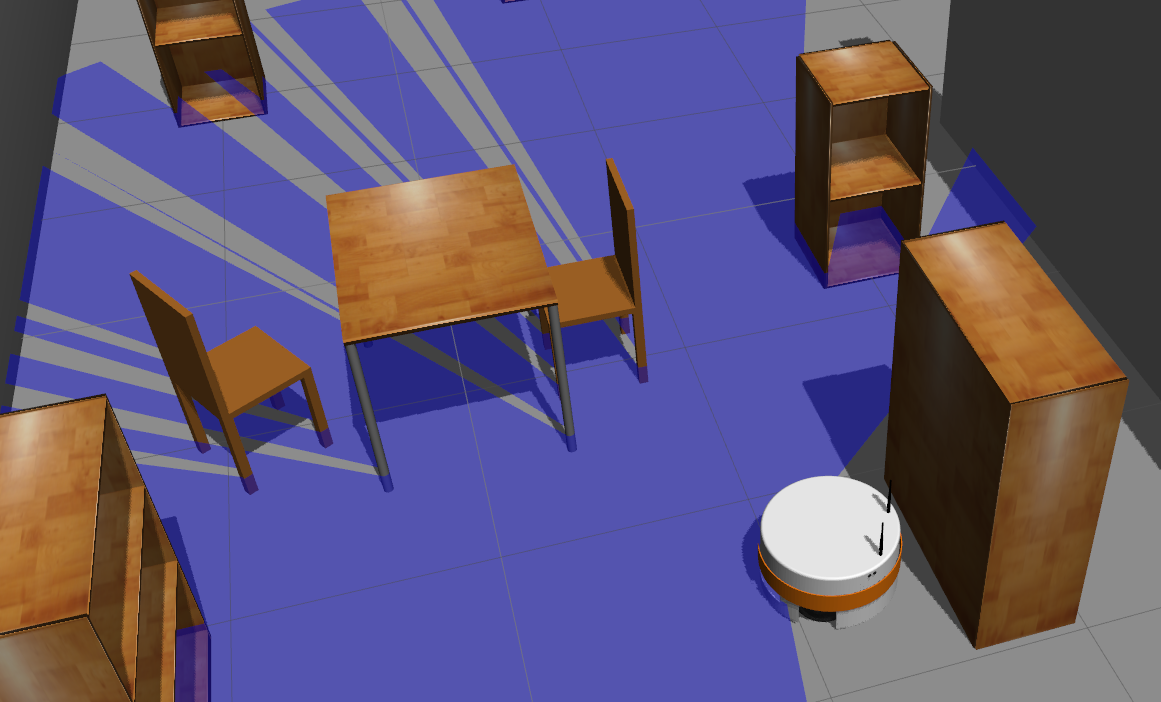
\includegraphics[width=0.5\textwidth]{imgs/gazebo2.png}
\label{fig:gazebo2}
\caption{Gazebo Environment}
\end{figure}

Ros integrates closely with Gazebo through the $gazebo\_ros$ package. The latter provides a Gazebo plugin module that allows bidirectional communication between ROS and the simulator. Sensors, physics data, video input can stream from Gazebo to ROS and actuators commands can be forwarded to the simulation environment. By choosing consistent names and data types for these data streams it is possible to run the low level device-driver software on both the real robot and in the simulator. In this project Gazebo 8.0 and ROS Indigo have been used. This combination ensures the compatibility required to flawlessly run the application.
\section{The Architecture}

This project has been implemented using ROS framework. It is a modular application that enables other nodes to query and interact with the knowledge base. An external interface node allows several operations including the export of the Assertion Box. Four nodes are involved in this application and the communication between them relies on an inter-process protocol handled by ROS.

\subsection{System description}
In the following subsection, the implememted nodes and their interaction with the system will be discussed. 

\begin{figure}[H]
\centering
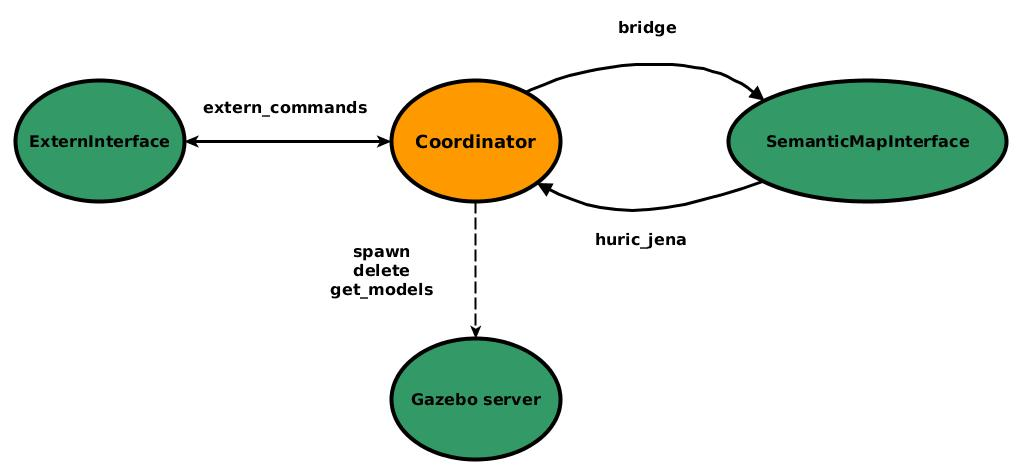
\includegraphics[width=0.8\textwidth]{imgs/arch1.jpg}
\label{fig:actions}
\caption{System Architecture}
\end{figure}

\subsubsection{SemanticMapInterface Node}
The knowledge base is loaded from the SemanticMapInterface which is a Java node based on the Jena Ontology API. This process allows requesting nodes to access and manipulate the ontology using a predefined set of operations.

\begin{figure}[H]
\centering
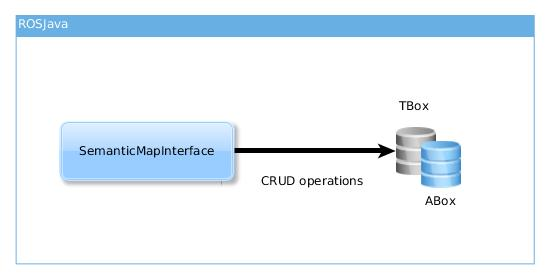
\includegraphics[width=0.8\textwidth]{imgs/semantic.jpg}
\label{fig:actions}
\caption{SemanticMapInterface Node}
\end{figure}

The exposed operations include:

\begin{itemize}
\item Loading the Terminology (TBox) and Assertion Box (ABox) into memory,
\item Listing instances, their spacial properties and their preferred lexical reference,
\item Adding a new entity of a particular class, with the spacial and lexical properties specified as arguments,
\item Updating properties of active entities,
\item Removing active entities,
\item Invoking OWL-FULL reasoner and performing inference operation given a domain model, 
\item Exporting in OWL format the list of instances present or the augmented ABox with derived properties.

\end{itemize}

\subsubsection{Gazebo Nodes}

Gazebo is a free (freedom) and open source robot simulation environment. It provides high performance physics engines to model real world dynamics, render 3D objects and environments. The Gazebo server \textit{gzserver} executes the simulation process including physics updates. The Gazebo client runs the UI and provides a 3D environment and handy controls to modify simulation properties. These nodes provide a set of ROS API's that allows users to modify and get information about various aspects of the simulated world.

Topics can be used to set the pose and twist of a model by publishing desired model state message to /gazebo/set\_model\_state\_topic. It is possible to retrieve model and link states using Topics. Gazebo publishes /gazebo/link\_states and /gazebo/model\_states\_topics, containing pose and twist information of objects in simulation with respect to the gazebo world frame. Services can be used to create/spawn and destroy models dynamically in simulation.

\subsubsection{Extern Interface Node}
This node has been implemented to test the required specifications. It simulates external requests by publishing predefined encoded messages on a topic to which the Coordinator is subscribed. The supported operation are listed in section \ref{sec:objectives}


\subsubsection{Coordinator Node}
The Coordinator node is a python script that performs several actions and communicates with other nodes in the system. One responsability of the coordinator is to keep track of instances and trigger update requests when a 3D model is manually grabbed and moved in the simulation. This node provides a dynamic rooting of requests from the External Interface node to the ontology handler or Gazebo. 

Basic operations include:

\begin{itemize}
\item Handles high level requests from other nodes such as visualizing or exporting the  list of instances present in the ontology.
\item Tracks 3D absolute positions of objects in the simulation,
\item Notifies the ontology manager that an instance's property has changed,
\item Forwards 3D spawn and delete task to Gazebo,
\item Ensures consistency bewteen the Assertion Box and the simulated world.
\end{itemize}

\subsection{Test cases}

The following test cases have been performed:

\begin{itemize}
\item Initialization from non empty ontology (TBox and ABox),
\item Retrieve collection of intances and render 3D models in Gazebo,
\item Request a detailed list of properties about active entities,
\item Manually drag objects in scene and sync new properties with the ABox,
\item Request Instances enumeration from ExternalInterface,
\item Perform a consistency check.
\item Requests:
	\begin{itemize}
		\item Deletion of entities,
		\item Insertion of default instance,
		\item Insertion of instance with specified type, spacial and lexical property,
		\item Export to specified file.
	\end{itemize}
\end{itemize}
\section{The Application}

The application consists of a number of indipendent nodes that comprise a graph. The communication between nodes strongly relies on a publish/subscribe mechanism useful to  exchange data in a distributed system. 

\subsection{Use cases}

\subsubsection{Initialization}
The application is launched by executing the init.launch file. The Roslaunch tool allows to launch multiple ROS nodes as well as set several parameters for the simulation environment. the initialization process brings up the master node, roscore, the coordinator, the semanticMapInterface and Gazebo.\\
\\
Once initialized, the SemanticMapInterface loads from a specified absolute path the Terminology Box and the Assertions Box as Ontology Models.

\begin{lstlisting}[language=Java]
/**
 * Importing Tbox
 */
 tbox = ModelFactory.createOntologyModel( OntModelSpec.OWL_MEM );
 OntDocumentManager dm_tbox = tbox.getDocumentManager();
 dm_tbox.addAltEntry(SOURCE+TBOX_FILE,"file:"+TBOX_FILE);
 tbox.read(SOURCE+TBOX_FILE,"RDF/XML");

/**
 * Importing Abox
 */
 abox = ModelFactory.createOntologyModel( OntModelSpec.OWL_MEM);
 OntDocumentManager dma = abox.getDocumentManager();
 dma.addAltEntry( SOURCE + ABOX_FILE , "file:" + ABOX_FILE);
 abox.read(SOURCE + ABOX_FILE,"RDF/XML");
\end{lstlisting}

The reasoner API supports the notion of specializing a reasoner by binding it to a set of schema or ontology data using the bindSchema call. The specialized reasoner can then be attached to different sets of instance data using bind calls. It is worth noting that in this project the schema (TBox) and instance (ABox) data were saved in two separate files.

\begin{lstlisting}[language=Java]
Reasoner reasoner = ReasonerRegistry.getOWLReasoner();
reasoner = reasoner.bindSchema(tbox);
OntModelSpec ontModelSpec=OntModelSpec.OWL_MEM_MICRO_RULE_INF;
ontModelSpec.setReasoner(reasoner);
InfModel infmodel = ModelFactory.createInfModel(reasoner,abox);
\end{lstlisting}
This is equivalent to an Ontology Model with Reasoner capabilities
specialized on the ABox.
\begin{lstlisting}[language=Java]
infModel = ModelFactory.createOntologyModel( OntModelSpec.OWL_MEM_MICRO_RULE_INF, abox);
\end{lstlisting}

Typically the ontology languages used with the semantic web allow constraints to be expressed, the validation interface is used to detect when such constraints are violated by some data set. The InfModel.validate() interface performs a global check across the schema and instance data looking for inconsistencies. 


\begin{lstlisting}[language=Java]
/** 
 * Consistency Check. Returns true if passed
 */
 private static boolean performConsistencyCheckWith(InfModel inf) {
 boolean res = false; 

 ValidityReport validity = inf.validate();
 if (validity.isValid()) {
	System.out.println(""+ NODE_NAME + "\tConsistency Check:\n Passed\n");
	res = true;
 } else {
	System.out.println(""+ NODE_NAME + "\tConsistency Check:\n Conflicts\n");
	for (Iterator i = validity.getReports(); i.hasNext(); ) {
	    System.out.println(" - " + i.next());
	}
 }
 return res;
}
\end{lstlisting}

When the Coordinator is initialized it sends on a topic called Bridge an init request. The request is captured by the SemanticMap and the $getAllInstances(OntModel)$ method is called. 

\begin{figure}[H]
\centering
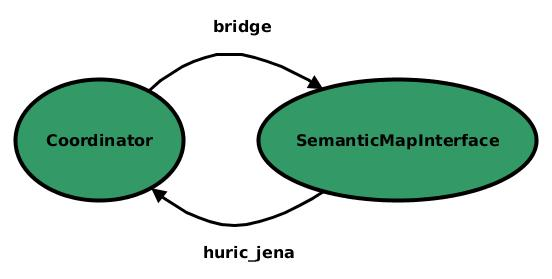
\includegraphics[width=0.8\textwidth]{imgs/topics1.jpg}
\label{fig:actions}
\caption{Data exchange between Coordinator and SemanticMapInterface}
\end{figure}


A collection of instances is retrieved and saved in a HashMap. This method performs the following SPARQL query which returns all Furniture and Drink\footnote{Furniture and Drink are classes defined in the Terminology Box} entities. 

\begin{lstlisting}[language=Java]
String queryString = "PREFIX rdf: <http://www.w3.org/1999/02/22-rdf-syntax-ns#>" +
				"prefix rdfs: <"+RDFS.getURI()+">\n" +
	    		"PREFIX xsd: <http://www.w3.org/2001/XMLSchema#> " +
	    		"PREFIX hasPosition: <" + NS + POSITION +"> " +
	    		"PREFIX hasRef: <" + NS + PREF_REF +"> " +
				"prefix semantic_mapping_domain_model: <" + DOMAIN_MODEL_NS + "#> \n"+
				"prefix semantic_mapping_1: <" + SEMANTIC_MAP_NS + "#> \n"+
	    		
	    		"PREFIX coordx: <" + NS + COORD_X +"> " +
	    		"PREFIX coordy: <" + NS + COORD_Y +"> " +
	    		"PREFIX coordz: <" + NS + COORD_Z +"> " +
	    		"PREFIX prefRef: <" + NS + LEXICAL +"> " +
	    		
	    		
	    		"SELECT DISTINCT ?uri ?class ?x ?y ?z ?lex "+
	    		"WHERE {" + 
	    			"{"+
		    		"?uri a ?class ." + 
		    		"?class rdfs:subClassOf semantic_mapping_domain_model:Furniture ."+
		    		"?uri hasPosition: ?pos ." + 
		    		"?uri hasRef: ?ref ." + 
		    		"?ref prefRef: ?lex ." + 
		    		"?pos coordx: ?x . " + 
		    		"?pos coordy: ?y . " + 
		    		"?pos coordz: ?z " +  "} UNION {"+
		    		"?uri a ?class ." + 
		    		"?class rdfs:subClassOf semantic_mapping_domain_model:Drink ." +
		    		"?uri hasPosition: ?pos ." + 
		    		"?uri hasRef: ?ref ." + 
		    		"?ref prefRef: ?lex ." + 
		    		"?pos coordx: ?x . " + 
		    		"?pos coordy: ?y . " + 
		    		"?pos coordz: ?z " +  "}"+
"}" ;
\end{lstlisting}
The resulting information are embedded in a message and sent on a topic called \textit{Huric\_jena}. The Coordinator Node receives and parses the message. 

The communication between Gazebo and the Coordinator uses services which are defined as pair of messages: one for the request and one for the reply. A providing ROS node offers a service under a string name, and a client calls the service by sending the request message and awaiting the reply.

Once the reponse from the SemanticMapInterface has been received, the Coordinator calls a special service that allows to create and render 3D models dynamically in the simulation environment of Gazebo.


\begin{figure}[H]
\centering
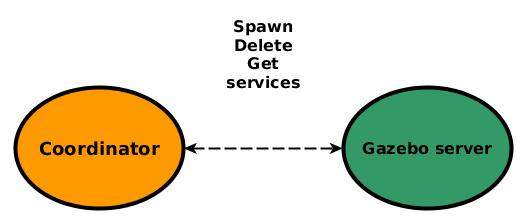
\includegraphics[width=0.5\textwidth]{imgs/gazebocoord.jpg}
\label{fig:actions}
\caption{Data exchange between the Coordinator and Gazebo}
\end{figure}



\subsubsection{Insertion of entities}
\label{subsec: insertion}
Considering a real world scenario in which a perception node recognizes an object from a stream of a point cloud data, instances of a given class should be dynamically inserted in the Assertion Box by publishing a predefined command on a topic.\\
One node can create an instance by specifying its super class, its spacial positions and preferred lexical reference. Another faster way include the possibility to add a Chair in fixed position. These insertion methods are issued by the ExternInterface node, captured by the Coordinator and forwarded to the SemanticMapInterface.


\begin{figure}[H]
\centering
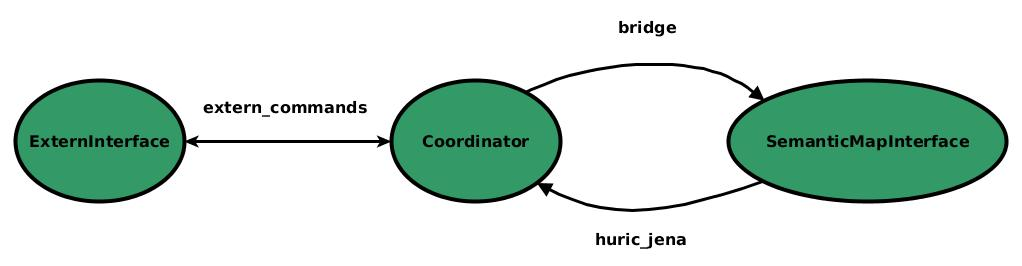
\includegraphics[width=0.8\textwidth]{imgs/topics2.jpg}
\label{fig:actions}
\caption{Data exchange between ExternInterface, Coordinator and SemanticMapInterface}
\end{figure}


The Java Node provides two methods to insert an instance of given type into the ontology model loaded in memory:
\begin{itemize}
\item Triple manipulation based
\item SPARQL based
\end{itemize}
Jena Ontology API provides a full set of methods to manipulate statements. The handleAddEntityRequest(ontModel,ontClass, uri, pose,lexicalReference) method is given below:

\begin{lstlisting}[language=Java]
/**
 * Handles AddEntityRequests from orchestrator using Jena API
 *	Creates a new instance, adds properties to it and perform consistency check
 * If test is passed, leaves the newly created instance, otherwise deletes it
 */
	private static boolean handleAddEntityRequest(OntModel abox, OntClass ontClass, String uriInstance, String posX,
			String posY, String posZ, String lexicalReference){
		boolean res = false;

	    OntClass prefrefClass = abox.getOntClass(NS+PREF_REF_CLASS);
	    OntClass coordinatesClass = abox.getOntClass(NS+COORDINATES_CLASS);

		String uriBase = "http://www.semanticweb.org/ontologies/2016/1/semantic_mapping_1#";
		// Create instance
	    //OntClass class1 = abox.getOntClass(NS+ontClass);
		
		if (ontClass == null)
			return false;
		else {
			// Create Individuals
			Individual i1 = abox.createIndividual(uriInstance,ontClass);
		    Individual prefRefInd = abox.createIndividual(uriBase+lexicalReference
		    +"_pref_ref",prefrefClass);
		    Individual coordinatesInd = abox.createIndividual(uriBase+lexicalReference
		    +"_pref_ref",coordinatesClass);
			
			
		    // Create Datatype Property
		    DatatypeProperty lexicalRef = abox.getDatatypeProperty(NS + LEXICAL);
			Literal ref = abox.createTypedLiteral(lexicalReference);
			Statement refStatement = abox.createStatement(prefRefInd, lexicalRef, ref);
			abox.add(refStatement);
			
			//  Bind pref reference individual to object individual
			ObjectProperty hasPrefRef = abox.getObjectProperty(NS+PREF_REF);
			Statement bindPrefRef = abox.createStatement(i1, hasPrefRef, prefRefInd);
			abox.add(bindPrefRef);
			

		    // Create Datatype Property for coordinate X
		    DatatypeProperty posx = abox.getDatatypeProperty(NS + COORD_X);
			Literal posXFloat = abox.createTypedLiteral(posX);
			Statement posXStatement = abox.createStatement(coordinatesInd, posx, posXFloat);
			abox.add(posXStatement);
		    // Create Datatype Property for coordinate X
		    DatatypeProperty posy = abox.getDatatypeProperty(NS + COORD_Y);
			Literal posYFloat = abox.createTypedLiteral(posY);
			Statement posYStatement = abox.createStatement(coordinatesInd, posy, posYFloat);
			abox.add(posYStatement);
		    // Create Datatype Property for coordinate X
		    DatatypeProperty posz = abox.getDatatypeProperty(NS + COORD_Z);
			Literal posZFloat = abox.createTypedLiteral(posZ);
			Statement posZStatement = abox.createStatement(coordinatesInd, posz, posZFloat);
			abox.add(posZStatement);
			

			//  Bind position individual to object individual
			ObjectProperty hasPosition = abox.getObjectProperty(NS+POSITION);
			Statement bindPose = abox.createStatement(i1, hasPosition, coordinatesInd);
			abox.add(bindPose);
			
			// Now perform consistency check

		    InfModel infModel = ModelFactory.createOntologyModel( OntModelSpec.OWL_MEM_MICRO_RULE_INF, abox);
			res = performConsistencyCheckWith(infModel);
		}
		
		return res;
}
\end{lstlisting}

The second method is called AddEntityRequest(abox,ontclass,uri,pose,lexicalReference) and it is based on a SPARQL query:

\begin{lstlisting}[language=Java]
/**
 * Handles AddEntityRequests using SPARQL
 *	Creates a new instance, adds properties to it and perform consistency check
 * If test is passed, leaves the newly created instance, otherwise deletes it
 */
 private static boolean AddEntityRequest(OntModel abox, OntClass ontClass, String uriInstance, String posX,
			String posY, String posZ, String lexicalReference){
 boolean res = true;
		
 String uri_Instance[] = uriInstance.split("#");
		
 if (ontClass == null) {
    res = false;
	System.out.print("\n"+ NODE_NAME + "\t[ Add Entity ] Class problem\n");
 } else {
			String queryString = "" + 
			"prefix rdfs: <"+ RDFS.getURI() +">\n" +
			"prefix rdf: <http://www.w3.org/1999/02/22-rdf-syntax-ns#> \n"+
			"PREFIX xsd: <http://www.w3.org/2001/XMLSchema#> "
			
			+ "prefix semantic_mapping_domain_model: <" + DOMAIN_MODEL_NS + "#> \n"
			+ "prefix semantic_mapping: <" + SEMANTIC_MAP_NS + "#> \n"
			+ "PREFIX class: <"+ ontClass.getURI() +">\n"
			
			
			+ "insert data { semantic_mapping:"+uri_Instance[1] +" rdf:type class: . "
			
			
			// Add hasPosition Irreflexive ObjectProperty 
			+ "semantic_mapping:" + uri_Instance[1] + " semantic_mapping_domain_model:hasPosition semantic_mapping:" + uri_Instance[1]
			+ "_coordinates . " 
			
			// Add Instance Coordinates 
			+ "semantic_mapping:" + uri_Instance[1]+ "_coordinates rdf:type semantic_mapping_domain_model:Coordinates . " 

			// Add datatype Property
			+ "semantic_mapping:" + uri_Instance[1] + "_coordinates semantic_mapping_domain_model:float_coordinates_x \""
			+ posX + "\"^^xsd:float . "
			+ "semantic_mapping:" + uri_Instance[1] + "_coordinates semantic_mapping_domain_model:float_coordinates_y \"" + posY
			+ "\"^^xsd:float . "
			+ "semantic_mapping:" + uri_Instance[1] + "_coordinates semantic_mapping_domain_model:float_coordinates_z \"" + posZ
			+ "\"^^xsd:float . "

			// Add hasPreferredReference ObjectProperty
			+ "semantic_mapping:" + uri_Instance[1] + " semantic_mapping_domain_model:hasPreferredReference semantic_mapping:" + uri_Instance[1]
			+ "_preferredReference . " 

			// Create Instance Lexical Reference
			+ "semantic_mapping:" + uri_Instance[1] + "_preferredReference rdf:type semantic_mapping_domain_model:PreferredReference . "

			+ "semantic_mapping:" + uri_Instance[1] + "_preferredReference semantic_mapping_domain_model:lexicalReference \"" + lexicalReference
			+ "\"^^xsd:string . " + "} \n ";
			
			UpdateAction.parseExecute(queryString, abox);
			
			// Check inconsistencies
		    InfModel infModel = ModelFactory.createOntologyModel( OntModelSpec.OWL_MEM_MICRO_RULE_INF, abox);
			res = performConsistencyCheckWith(infModel);
		}
	
		return res;
}
\end{lstlisting}

Once the instance has been inserted into the ontology model, the collection of new entities is once again sent on the \textit{huric\_jena} topic and captured by the coordinator which invokes the Gazebo service to render the 3D model of the newly created instances at the provided position in space.


\subsubsection{Deletion of an entity}
\label{subsubsec:delete}
In a real world scenario, objects can move or be manipulated by humans. A delete function is needed in order to handle cases in which the object moves out of the field of perception of the robot. To delete a model a special routine is invoked.\\
The request is published on the external\_commands topic and captured by the Coordinator. This node forwards the request to SemanticMapInterface node and waits for the response. If the abox has been correctly updated, it invokes the delete\_model service exposed by the Gazebo node. The resulting 3D environment is consistent with the instance data loaded in memory.

The SemanticMapInterface provides a method the handle this request. In Section \ref{subsec:abox} we have seen that for each furniture object there is an linear position and lexical reference instance associated with it. In order to completely delete a furniture object, these instances have to be cancelled as well. The query that handles this operation is in the Listing below.
\begin{lstlisting}[language=Java]
/**
  * Handles removeEntityRequests from orchestrator:
  *	Looks for an instance with uri 'uriInstance', if the instance does not exist returns flase.
  * If there is match, it deletes it and returns true. 
  * 
  * Attention : What happens if an instance of a master concept relating two entities is deleted?
  * 			No one should be able to alter its knowledge directly.
  *	
  * 			Maybe, add a negative weight to the instance or a tag
  */
private static boolean handleRemoveEntityRelatedRequest(OntModel abox, String uriInstance) {
	boolean res = false;

	String uri_Instance[] = uriInstance.split("#");
	//  Removing IS A statement
	String queryStringDelete = "" + 
			"prefix rdfs: <"+RDFS.getURI()+">\n" +
			"prefix rdf: <http://www.w3.org/1999/02/22-rdf-syntax-ns#> \n"+
			"PREFIX xsd: <http://www.w3.org/2001/XMLSchema#> "				
			+ "prefix semantic_mapping_domain_model: <" + DOMAIN_MODEL_NS + "#> \n"
			+ "prefix semantic_mapping: <" + SEMANTIC_MAP_NS + "#> \n"
			+ "delete { semantic_mapping:"+uri_Instance[1] +" ?pred ?obj }  "
        + "where { semantic_mapping:"+uri_Instance[1] + " ?pred ?obj }";
			
			UpdateAction.parseExecute(queryStringDelete, abox);
	

	//  Removing coordinates statement
	String queryStringPosDelete = "" + 
			"prefix rdfs: <"+RDFS.getURI()+">\n" +
			"prefix rdf: <http://www.w3.org/1999/02/22-rdf-syntax-ns#> \n"+
			"PREFIX xsd: <http://www.w3.org/2001/XMLSchema#> "				
			+ "prefix semantic_mapping_domain_model: <" + DOMAIN_MODEL_NS + "#> \n"
			+ "prefix semantic_mapping: <" + SEMANTIC_MAP_NS + "#> \n"
			+ "delete { semantic_mapping:"+uri_Instance[1] + "_coordinates ?pred ?obj }  "
        + "where { semantic_mapping:"+uri_Instance[1] + "_coordinates ?pred ?obj }";
			
			UpdateAction.parseExecute(queryStringPosDelete, abox);
	
	String queryStringRefDelete = "" + 
			"prefix rdfs: <"+RDFS.getURI()+">\n" +
			"prefix rdf: <http://www.w3.org/1999/02/22-rdf-syntax-ns#> \n"+
			"PREFIX xsd: <http://www.w3.org/2001/XMLSchema#> "				
			+ "prefix semantic_mapping_domain_model: <" + DOMAIN_MODEL_NS + "#> \n"
			+ "prefix semantic_mapping: <" + SEMANTIC_MAP_NS + "#> \n"
			+ "delete { semantic_mapping:"+uri_Instance[1] + "_preferred_reference ?pred ?obj }  "
        + "where { semantic_mapping:"+uri_Instance[1] + "_preferred_reference ?pred ?obj }";
			
			UpdateAction.parseExecute(queryStringRefDelete, abox);
			
	return res;
}
\end{lstlisting}
\label{lst:delete}

\subsubsection{Update entity's properties}
The system provides an update function to modify properties of an existing entity in the ABox. By publishing a formatted command on the extern\_commands topic, the Coordinator node forwards the request to the SemanticMapInterface. The method responsible for the update is called handleUpdateEntityRequest(abox,ontClass, uriInstance, posX, posY, posZ,  lexicalReference).

\begin{lstlisting}[language=Java]
/**
  * Handles updateEntityRequests using SPARQL
  *	Looks for an instance with uri 'uriInstance', if the instance does not exist returns flase.
  * If there is match, it looks for the properties Pose and LexicalReference and updates it. 
  * A consistency if invoked. If the test is passed, true is returned. Otherwise False.
  */
private static boolean handleUpdateEntityRequest(OntModel abox,OntClass ontClass,
 String uriInstance, String posX,
		 String posY, String posZ, String lexicalReference) {
	boolean res = false;

	System.out.println(""+ NODE_NAME + "\tDeleting Instance " + uriInstance);
	handleRemoveEntityRelatedRequest(abox,uriInstance);

	System.out.print("\n"+ NODE_NAME + "\tNow inserting: "+ posX + ", " + posY + " , " + posZ);
	if (AddEntityRequest(abox,ontClass,uriInstance,posX,posY,
	posZ,lexicalReference)) {
	System.out.println("\n"+ NODE_NAME + "\tInstance inserted successfully");
	res = true;
   	} else {
    		System.out.print(""+ NODE_NAME + "\tError could not insert instance consistency problem");
    	}
	
	return res;
}
\end{lstlisting}

The update routine starts by looking for an instance with the provided uri. If the there is no match, false is returned. Then it deletes the instance itself and its related properties with the method presented in Section \ref{subsubsec:delete}. Finally the new instance is added by invoking the method discussed in Section \ref{subsec: insertion} and a consistency check is invoked. 

It is also possible to update an instance by dragging it in the 3D environment of Gazebo. The coordinator node keeps track of the position of all instances and compare them with the correponding coordinate properties in the Assertion Box. As soon as the position of an instance is modified and a customizable threshold is crossed, an update routine is triggered and the ABox is updated. Collisions have not been taken into account.

\subsection{Exporting Ontology}
Human machine interfaces require a context-aware interaction. In this process, since both parts make references to real world objects, an ontological model of the environment and a description of the involved entities may help in improving the accuracy of the interpretation of an user utterance.\\
The first step towards this direction is to provide an export feature that allows the robotic platform to be aware of the surrounding environment and nearby objects.\\
\\

\begin{lstlisting}[language=Java]
/** 
  * Exports Ontology if consistency check passed
  */
private static boolean exportTo(InfModel inf, OntModel abox, String absolutePath, String fileName){
	boolean res = false;
	if (performConsistencyCheckWith(inf)) {
		exportOntologyOnt(abox,absolutePath,fileName);
		res = true;
	}
	else {
		res = false;
	}
	return res;
}

/** 
  * Exports Ontology to a file with provided name and path.
  */
private static boolean exportOntologyOnt(OntModel inf, String absoluteFileName, String fileName){
	boolean res = false;
    FileWriter out = null;

    	try{
    		out = new FileWriter(absoluteFileName+fileName);
    		inf.write(out,"RDF/XML-ABBREV");
    		res = true;
	    	System.out.println(""+ NODE_NAME + "\tConsistency check passed. Writing to file:\t"+fileName);
    	}
    	catch (IOException a){
    		System.out.println(""+ NODE_NAME + "\tExport Problem");
            a.printStackTrace();
    	}
    	finally{
    		if (out!=null){
    			try {out.close();} catch(IOException ex) {}
    		}
    	}

    	return res;
}
\end{lstlisting}

The SemanticMapInterface export the ontology to OWL file in the file system and sends the list of entities to the Coordinator Node.

\subsubsection*{Listing Entities}
\label{subsubsec:list}
In order to retrieve the list of entities perceived by the robot, another feature has been taken into account. This action involves the Coordinator, the SemanticMapHandler and the ExternInterface nodes. The Coordinator prepares the response in two formats, a json encoded list of entities and corresponding properties

\begin{lstlisting}[language=Java]
{
   "http://www.semanticweb.org/ontologies/2016/1/semantic_mapping_1#table1":{
      "type_full":"http://www.semanticweb.org/ontologies/2016/1/semantic_mapping_domain_model#Table",
      "coordinates":"2.0,2.0,0.0",
      "preferredLexicalReference":"table",
      "atom":"table1",
      "coordinate":{
         "y":"2.0",
         "x":"2.0",
         "z":"0.0"
      },
      "type":"Table"
   },{
   ...
   },
   "http://www.semanticweb.org/ontologies/2016/1/semantic_mapping_1#beer_can_1":{
      "type_full":"http://www.semanticweb.org/ontologies/2016/1/semantic_mapping_domain_model#Beer",
      "coordinates":"1.8,2.2,1.0",
      "preferredLexicalReference":"Beer",
      "atom":"beer_can_1",
      "coordinate":{
         "y":"2.2",
         "x":"1.8",
         "z":"1.0"
      },
      "type":"Beer"
   }
}
\end{lstlisting}


and human readable output for debug purposes.  




\subsection{Future works}

The application described supports a limited number of entity's types. Each instance has to be associated with its corresponding 3D model with correct inertia matrix. In this project four types of objects are supported: tables, chairs, beer and coke cans.

From a robotic perspective, the applications of this ROS package are related to Human Centered Robotics and Machine to Machine Interaction.

\subsubsection{LU4R - Adaptive spoken Language Understanding For Robots}
The adaptive spoken Language Understanding chain For Robots tool is the result of the collaboration between the SAG group at Tor Vergata University of Rome and the Laboratory of Cognitive Cooperating Robots (Lab.Ro.Co.Co.) at Sapienza, University of Rome. LU4R\footnote{For further information visit the official webpage at http://sag.art.uniroma2.it/lu4r.html} receives as input one or more transcriptions of a spoken command and produces an interpretation that is consistent with a linguistically-justified semantic representation, coherent with the perceived environment. Lu4r is based on a spoken language understanding (SLU) process that integrates perceptual and linguistic informationin order to produce command interpretations that coherently express constraints about the world and the hosting robotic platform.\\
\\
It is a ROS compatible Java application in which the client runs on the robotic platform and the server on a remote machine.\\
Actions expressed in user utterances can be modeled as semantic frames, sentences expressing commands are automatically analyzed by the chain by applying data driven methods trained over the Human Robot Interaction Corpus (HuRIC)\cite{bib3}.
\\
In its default mode of operation, the chain requires a list of sentences paired with their transcription confidence score. Each entry corresponds to a speech recognition hypothesis. 
%In order to react to a user command a number of implicit assumptions should be made. 

%The correct interpretation of the spoken sentences depends on the physical, cognitive and linguistic aspects triggered by the operational environment.

%``take the book on the table ''

%First, at least two entities, a book and a table, must exist in the environment and the speaker must be aware
%of such entities. Accordingly, the robot must have access to
%an inner representation of the objects, e.g. an explicit map of
%the environment.
%The perception of the environment that explicitly affects linguistic reasoning.
%In the ontology based approach, OWL is used to model a Reference Ontology, while RDFS  is used  to  model schemas  to  be mapped. 


The following points assume that the robot is equipped with a spoken command recognition

Lu4r

PointCloud

% ELENCO DELLE FIGURE (OPZIONALE)
\addcontentsline{toc}{chapter}{Elenco delle figure}
\listoffigures


% BIBLIOGRAFIA
\addcontentsline{toc}{chapter}{References}
\begin{thebibliography}{11}
	
	\bibitem{bib1} E. Bastianelli, D. D. Bloisi, R. Capobianco, F. Cossu,
G. Gemignani, L. Iocchi, and D. Nardi,
            \emph{``On-line semantic mapping''} in 16th International Conference on Advanced
Robotics, Nov 2013.

	\bibitem{bib2} Emanuele Bastianelli, Danilo Croce, Roberto Basili, Daniele Nardi,
            \emph{``Using Semantic Maps for Robust Natural Language Interaction with Robots''}, DICII, 2 DII - University of Rome Tor Vergata, DIAG - Sapienza University of Rome - Rome, Italy.

	\bibitem{bib3} Emanuele Bastianelli, Giuseppe Castellucci, Danilo Croce, Luca Iocchi, Roberto Basili, Daniele Nardi,
            \emph{``HuRIC: a Human Robot Interaction Corpus''} 

	\bibitem{bib4} E. Bastianelli, Giuseppe Castellucci, Danilo Croce, Roberto Basili, Daniele Nardi,
            \emph{``Effective and Robust Natural Language Understanding
for Human -R obot Interaction''}, ECAI, 2014.
	
	\bibitem{bib5} E. Bastianelli, D. Bloisi, R. Capobianco, G. Gemignani, L. Iocchi, D. Nardi,
            \emph{``Knowledge Representation for Robots through
Human-Robot Interaction''}, Rome.

	\bibitem{bib6} Aaron Martinez, Enrique Fern\'andez,
            \emph{``Learning ROS for Robotics Programming''} A practical, instructive, and comprehensive guide to introduce yourself to ROS, the top-notch, leading robotics framework, 2013.
            
    \bibitem{bib7} Lentin Joseph,
            \emph{``Learning Robotics Using Python''} Design, simulate, program, and prototype an interactive autonomous mobile robot from scratch with the help of Python, ROS, and Open-CV!, 2015.
            
    \bibitem{bib8} Lentin Joseph,
            \emph{``Mastering ROS for Robotics Programming''}, 2015 Packt Publishing.
                  
    \bibitem{bib9} Morgan Quigley, Brian Gerkey and William D. Smart,\\
            \emph{``Programming Robots with ROS''}, 2016 O Reilly Media.
                     
    \bibitem{bib10} Open Source Robotics Foundation,\\
            \emph{``GazeboSim documentation''}, http://gazebosim.org/tutorials, 2016.
                       
    \bibitem{bib11} R. Brachman, H. Levesque,\\
            \emph{``Knowledge Representation and Reasoning''}.
            
    \bibitem{bib12} Open Source Robotics Foundation, Ros Documentation,\\
            \emph{``$http://wiki.ros.org/rosjava_build_tools/Tutorials/hydro$''}.
            
    \bibitem{bib13} Jena Ontology Api, \\
            \emph{``https://jena.apache.org/documentation/ontology/''}.
            
    \bibitem{bib14} Jena Reasoner and Inference documentation,\\
            \emph{``http://jena.apache.org/documentation/inference/index.html''}.
            
            
    \bibitem{bib15} Apache Jena Fuseki standalone server documentation,\\
            \emph{``$https://jena.apache.org/documentation/serving_data/$''}.
            

    \bibitem{bib16} Point Cloud Library Documentation, \\
            \emph{``http://pointclouds.org/documentation/tutorials/index.php''}.            
          
            
            
            
    

        
\end{thebibliography}
\end{document}
